\begin{abstract}
Integrated scheduling of processing and transport in flexible job shops usually treats travel times as a constant matrix indexed by location, i.e.\ it assumes that vehicles do not interfere with one another.
When a finite fleet shares a sparse corridor network, travel time is no longer fixed data but the outcome of routing decisions (in this paper, routing means conflict-free path planning of vehicles on the corridor network); one job's occupancy of a corridor affects the operation times of other jobs.
We study the following problem: in shops where transport takes longer than processing and congestion concentrates on a few shared corridors, each operation can be processed by one of several robotic arms that are homogeneous in capability but heterogeneous in efficiency, while AGVs must travel conflict-free on this network.
Machine flexibility turns this coupling into an operational trade-off: when the corridor to a fast arm is congested, a slower arm with better connectivity may be the better assignment. Prior work has not measured this trade-off by including it in the evaluation objective of the search.

We propose a \emph{closed-loop bilevel framework}: the upper level decides machine assignment and operation sequencing, and the lower level generates conflict-free paths by time-window reservation; routing information from the lower level enters the decisions in two ways.
The first is \emph{routing-in-the-loop evaluation} (the evaluation path): the fitness of each candidate solution is the makespan after conflict-free lower-level routing, so yielding delay enters the optimization objective of the search instead of serving only as a post-hoc check.
The second is \emph{reservation-table-aware dispatching} (the decision path): when a vehicle is selected, a trial query of both transport legs is run on the current reservation table, and the vehicle with the earliest actual delivery is chosen, instead of selecting a vehicle by travel times estimated under the assumption of an unimpeded trip.
To keep each dispatching evaluation \emph{low-overhead}, we give two speed-ups---admissible lower-bound pruning and winner-path reuse---and prove that they only reduce computation and change neither the selected vehicle nor the final timetable.

Experiments are run on \NCases{} controlled instances (contention intensity from \ContentionLo{} to \ContentionHi{}), with \NSeeds{} random seeds per instance, an equal wall-clock budget, and paired tests with multiple-comparison correction.
Starting from the open-loop structure in the literature (the search ignores conflicts, and vehicles are dispatched by unimpeded travel time), the complete method reduces the realized makespan by \GainEndToEnd{} (\WinEndToEnd{} wins, \LoseEndToEnd{} losses).
Most of the reduction comes from the closed loop: with the dispatching rule fixed and only the search made to count conflict-induced delay, makespan already falls by \GainLoopRule{}, and the reduction is significant per instance on the vast majority of instances; reservation-table-aware dispatching is a much smaller effect, significant only when all instances are pooled in one test. The two mechanisms each work on their own and do not amplify each other.
\end{abstract}

%%
%% The code below is generated by the tool at http://dl.acm.org/ccs.cfm.
%% Please copy and paste the code instead of the example below.
%%
%% 原有的 CCS 分类块描述的是上一篇论文(Robotic autonomy),与本文无关,故整块注释掉。
%% concept_id 由 dl.acm.org/ccs.cfm 的工具指派,不能手写,所以这里不填占位值。
%% 若最终投 ACM,请到该工具重新生成并粘回,建议选:
%%   Theory of computation~Scheduling algorithms            (significance 500)
%%   Applied computing~Industry and manufacturing           (significance 300)
%%   Computing methodologies~Planning and scheduling        (significance 300)
%% 投非 ACM 刊物时本块可直接删除。
%
% \begin{CCSXML}
% <ccs2012>...</ccs2012>
% \end{CCSXML}
% \ccsdesc[500]{Theory of computation~Scheduling algorithms}

%%
%% Keywords. The author(s) should pick words that accurately describe
%% the work being presented. Separate the keywords with commas.
\keywords{flexible job shop scheduling, conflict-free routing, closed-loop bilevel framework, routing-in-the-loop evaluation, reservation-table-aware vehicle dispatching}

%% ===================== 作者与单位 =====================
%% acmart 没有作者块会在编译时报 "No author given" 并把页眉留空。
%% 下面是占位:投稿前必须换成真实姓名、邮箱与单位,并按目标刊物的要求确认署名顺序。
%% 若目标会议要求双盲,改用 \documentclass[...,anonymous]{acmart},acmart 会自行遮蔽
%% 本块,不要手工把它删掉——删掉之后终稿会忘记加回来。
\author{Qi Yu}
%%\authornote{.}
%%\authornotemark[1]
\email{230240012@seu.edu.cn}
\orcid{0009-0008-7843-6345}
%%\authornote{corresponding author}
\affiliation{%
	\institution{School of Cyber Science and Engineering, Southeast University}
	\city{Nanjing}
	\state{Jiangsu}
	\country{PR China}
}
\author{Wei Li}
\orcid{0009-0001-0949-329X}
\email{xchlw@seu.edu.cn}
\authornote{corresponding author}
\affiliation{%
	\institution{School of Computer Science and Engineering, Southeast University}
	\city{Nanjing}
	\state{Jiangsu}
	\country{PR China}
}

%% 页眉用的短作者名,不填则 acmart 用 "Trovato et al."(模板残留)。
\renewcommand{\shortauthors}{Qi et al.}



%\Acknowledgements{This work was supported partly by Key Laboratory of Computer Network and Information Integration (Southeast University) of Ministry of Education of China under Grants NO. 93K-9 and Jiangsu Provincial Key Laboratory of Network and Information Security under Grants No.BM2003201.}


%% 三行收稿日期由编辑部回填。原先写的是 2025-11-27 收稿 / 2026-02-26 修回,
%% 早于本文数据的落盘日期,须在投稿时按实际提交日改写,不要沿用。
\received{XX XX 2026}
\received[revised]{XX XX 2026}
\received[accepted]{XX XX 2026}

%%
%% This command processes the author and affiliation and title
%% information and builds the first part of the formatted document.
\maketitle
\section{Introduction}
\label{sec:Chapter_I}

\subsection{Background and motivation}

Flexible job shop scheduling with transportation times has long rested on a convenient assumption: the time a job needs to move between two machines is a constant, read from a matrix indexed by location pairs.
This is the dominant convention in the literature~\cite{xin2025review}, and recent models still widely adopt it~\cite{meng2025cp,qin2026knowledge,fu2025integrated}.
The assumption is reasonable when the fleet is small enough relative to the corridor network that vehicles rarely meet.
Real shops, however, are not built that way: a few vehicles share a sparse corridor network, and a single-lane segment cannot be traversed in both directions at the same time; once fleet density is high enough, the fleet's own traffic turns from a secondary disturbance into the main cause of delay~\cite{kim2026congestion}.
Once this is acknowledged, travel time is no longer fixed data but the outcome of two decisions: the path a vehicle takes (we call this conflict-free path planning routing), and the order of reservations on contended segments.
The duration of a transport therefore has two parts: the travel time computed from distance, and the time spent waiting at berths or detouring because corridors are occupied by other vehicles. The latter means that one job's transport can delay the operations of other jobs.

Such delay, passed from job to job, leaves room for optimization only if the scheduler can adjust the assignment of operations, and machine flexibility is exactly what allows an operation to be reassigned to another arm (i.e.\ to change its processing location).
When an operation may be processed by any robotic arm in an option set, and the processing time depends on the chosen arm, the assignment decision selects both the destination and the processing duration.
Suppose an operation may be given either to a fast arm at the far end of the shop or to a slower arm right next to the load/unload point.
Under a constant travel-time matrix the comparison is arithmetic: a shorter processing time plus a longer travel time, against a longer processing time plus a shorter travel time.
With corridor contention it is different, because the corridor to the fast arm may be exactly the one that every other vehicle is using, and the waiting incurred there is invisible to the constant matrix.
A slower arm with better connectivity may then be the better choice; and at different congestion levels of the same instance, the conclusion may differ again.
This trade-off requires two ingredients at once: heterogeneous optional arms give the scheduler destinations it can switch between, and distinct paths in the corridor network make vehicles wait and detour differently on the way.

Figure~\ref{fig:motivating} uses a recomputable minimal instance to show that the same pair of assignments favours the fast arm when evaluated with a constant travel-time matrix, and the slow arm when evaluated with conflict-free routing.
The instance has $4$ jobs and $2$ AGVs: one operation of the focal job J1 may use M1 ($t^P=3$) or M2 ($t^P=14$); the other three background jobs can be processed only on M3; finished jobs must be returned to the load/unload point $v_0$.
The only route to the fast arm M1 is an exclusive trunk corridor, while the slow arm M2 lies on a separate branch; the background jobs cross the trunk repeatedly and keep it occupied.

The numbers in Figure~\ref{fig:motivating} are of two kinds: (a) the bottom gives the round-trip time of the focal job J1 on its own, used to determine the minimum difference in processing time between the fast and the slow arm; (b) the bar heights are the instance makespans when all four jobs are scheduled together, used to compare the assignment rankings produced by the two evaluation methods.
The bottom of Figure~\ref{fig:motivating}(a) gives J1's unimpeded round-trip time (outbound + processing + return): J1 leaves $v_0$ and is returned to $v_0$ after processing, with travel times taken from shortest paths and no other vehicles assumed on the way.
When J1 is assigned to M1, the path is $v_0\to v_1\to v_2\to\mathrm{M1}$, one way $1+\tau+1=8$, round trip $16$, plus processing $3$, giving $19$;
when J1 is assigned to M2, the path is $v_0\to v_1\to\mathrm{M2}$, one way $1+2=3$, round trip $6$, plus processing $14$, giving $20$.
Ignoring the other vehicles, the fast arm is better if and only if $19<6+t^P_{\text{slow}}$, i.e.\ $t^P_{\text{slow}}>13$; with $\tau=6$ and $t^P_{\text{fast}}=3$, this instance takes $t^P_{\text{slow}}=14$, so the two assignments differ by only $1$ and the fast arm wins by the smallest possible margin.
Only because the fast arm is better under unimpeded conditions does the choice of the slow arm under conflict-free routing, shown below, constitute a ranking reversal.

The bar heights in Figure~\ref{fig:motivating}(b) are the instance makespan $C_{\max}$, i.e.\ the time at which the last finished job returns to $v_0$, obtained by the same decoder as in the rest of the paper.
All four jobs start from $v_0$ and are returned to it; J2, J3, and J4 can be processed only on M3 (outbound and return legs $8$ each, processing $3$ each); the two AGVs can operate in parallel.

Under the constant matrix, vehicles do not interfere with one another, and yielding in corridors does not enter the evaluation.
If J1 is assigned to M1, then $C_{\max}=41$: in the first wave, J1$\to$M1 and J2$\to$M3 run in parallel, each with outbound $8$, processing $3$, and return $8$, and both are back at $v_0$ at $t=19$;
in the second wave, J3 and J4 are both transported to M3; they leave together at $t=19$ and arrive at $t=27$ after outbound $8$; J3 is processed during $27$--$30$ and returns at $38$, while J4 waits until M3 is free at $30$, is processed until $33$, and returns after another $8$, so the latest return time is $41$.
If J1 is assigned to M2, then $C_{\max}=54$: J1 has outbound $3$, processing $14$, and return $3$; AGV1 waits at M2 until $t=17$ and is back at $v_0$ at $t=20$; J2 still returns at $19$.
From then on the operations of the two vehicles are no longer synchronized; J4 arrives at M3 at $43$ and returns to $v_0$ at $54$. The matrix evaluation still chooses the fast arm.

Now the same pair of assignments is evaluated by conflict-free routing.
With J1 assigned to M1, $C_{\max}=95$: J1's own unimpeded round-trip time is still $19$, but its outbound leg occupies the trunk during $[1,7)$ and its return leg during $[12,18)$; J2 yields $17$ at the trunk entrance and arrives at M3 at $25$; J2--J4 then pass through the trunk one after another, and J4 returns to $v_0$ at $95$.
With J1 assigned to M2, $C_{\max}=60$: J1 takes the branch and does not occupy the trunk, and J2 yields only $1$ on $v_0$--$v_1$; the background jobs still yield to one another, and J4 returns to $v_0$ at $60$. The slow arm is now better.
Neither the machine assignment nor the operation sequence has changed; only the evaluation method has.

\begin{figure*}[t]
\centering
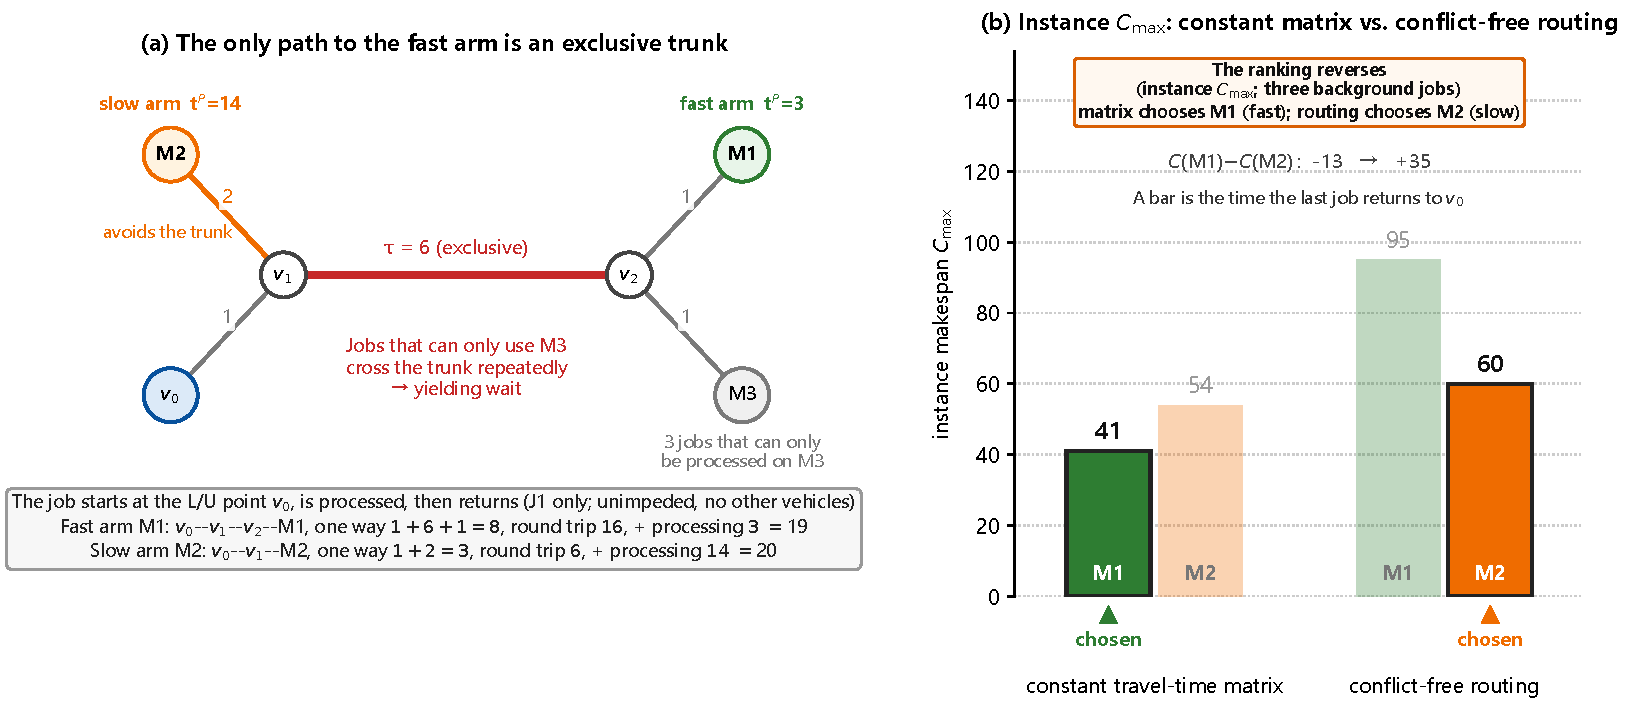
\includegraphics[width=\textwidth]{fig/fig_motivating.pdf}
\Description{Two panels. The left panel is a small shop network: the only route to the fast arm passes through an exclusive trunk, and the slow arm hangs on its own branch; the bottom gives the focal job's unimpeded round-trip times, 19 versus 20. The right panel shows the instance makespans of the same pair of assignments: under the constant matrix the fast arm wins, 41 versus 54; under conflict-free routing the result becomes 95 versus 60, and the slow arm wins.}
\caption{Motivating instance: the same assignment decision is ranked in opposite order by two evaluations.
(a) The only route to the fast arm M1 is an exclusive trunk ($\tau=6$); the slow arm M2 lies on a short corridor that does not pass through the trunk; three jobs that can be processed only on M3 cross the trunk repeatedly.
The bottom gives the unimpeded round-trip times of the focal job J1 (M1: $19$; M2: $20$), used to calibrate the minimum heterogeneity required for a reversal.
(b) Bar height is the instance makespan $C_{\max}$ ($4$ jobs, $2$ AGVs, same decoder as in the main text).
Under the constant matrix, $C_{\max}$ is $41$ versus $54$ and the fast arm is chosen; under conflict-free routing, the same pair of assignments gives $95$ versus $60$ and the slow arm is chosen, so the difference changes from $-13$ to $+35$.
This figure is an existence example; of the $1200$ parameter combinations around this instance, $205$ ($17\%$) show the reversal.}
\label{fig:motivating}
%% 由 fig/fig_motivating_CN.py 从 clbs/output/motivating.json 生成,后者由
%% clbs/tools/motivating.py --sweep 用与论文同一套解码器算出((b) 的四个数不是示意值:
%% 理想矩阵 = decode(conflict_free=False),无冲突路由 = decode(conflict_free=True))。
%% 算例:4 工件 / 3 机械臂 / 6 节点 / 5 走廊 / 2 AGV,delta_return=1,规则派车。
%% 注意:不要复用 fig/fig_intro_problem_new.pdf,那张图画的是上一篇论文
%% "邻近性对可用性"的场景,不是走廊争用。
\end{figure*}

\subsection{Gap relative to prior work}

A setting close to real AGV shops requires three conditions to hold at once: operations have optional machines, with processing times that depend on the machine; vehicles travel on an explicit road network with exclusive corridors, and travel times are determined jointly by the paths of all vehicles rather than taken from a constant matrix; and vehicles do not conflict with one another.
Most existing work covers only part of these: flexible job shop scheduling with transportation times represents travel by a constant travel-time matrix, and vehicles do not interfere with one another; conflict-free path planning handles vehicle travel, but the origins, destinations, and release times of tasks are given externally and do not change with the schedule.
Few works satisfy all three.
Van Os and Basten~\cite{vanos2026exact} formalize the problem as flexible job shop scheduling with conflict-free transportation constraints, and solve small benchmark instances to proven optimality with logic-based Benders decomposition.
This paper also studies flexible job shop scheduling with conflict-free routing, but focuses on a class of settings that prior work has not taken as a dedicated object of study: transport takes longer than processing ($\bar{T}_t/\bar{T}_p\approx4.0$, whereas common public instances reach at most \PubTtTpHi{}), robotic arms are connected by single-lane corridors, each corridor is exclusive over its whole length (van Os and Basten reserve nodes; see Section~\ref{sec:fjsppt}), vehicles may wait only at berths, and congestion concentrates on a few shared corridors.
In such shops, vehicle contention becomes the main constraint, and the quality of the same assignment changes with the level of congestion; we study this trade-off with contention intensity as a controlled variable, and target sizes that exact decomposition has difficulty solving.
At these sizes, existing heuristics either schedule first and resolve conflicts afterwards (Sun et al.~\cite{sun2023integrated}), or feed back the transport durations realized by the path layer once without modifying the assignment (Li et al.~\cite{li2026framework}), or embed routing in decoding without measuring its benefit and cost (Lyu et al.~\cite{lyu2019approach}).
Therefore, in this setting, it has not yet been measured under equal compute how the assignment should trade off between ``fast but congested'' and ``slow but clear'' arms, how much gain is obtained by counting yielding delay in the evaluation of the search, and at what level of contention this gain is worth its computational cost.

\subsection{Approach}

To address this gap, we adopt a bilevel structure: the upper level decides machine assignment and operation sequencing, and the lower level generates conflict-free paths by time-window reservation; routing information from the lower level enters the schedule in two ways, through evaluation and through decisions (detailed in the next two paragraphs), and we measure the contribution of each to makespan separately.

The \emph{evaluation path} takes the fitness of each candidate solution as the makespan after the lower level has completed conflict-free routing, so yielding wait enters the objective that the search optimizes, rather than serving as a post-hoc feasibility check.
One conflict-free decode costs more than an order of magnitude more computation than a decode based on unimpeded shortest-path times that ignore contention; under fixed compute, a higher cost per evaluation reduces the number of evaluations that can be completed.
Lyu et al.~\cite{lyu2019approach} already embed time-window routing in the decoding of a genetic algorithm, and Li et al.~\cite{li2026framework} list ``extending this into a fully iterative loop'' as future work, but neither reports the computational cost of this practice or its gain relative to open-loop scheduling. We measure this trade-off under an equal wall-clock budget.

The \emph{decision path} uses \emph{reservation-table-aware dispatching}. A transport consists of two legs: empty pickup and loaded delivery.
For each candidate vehicle, the lower-level router runs a trial query on the current reservation table for the earliest feasible times of the two legs in turn (the trial query does not write to the final timetable),
and the vehicle with the earliest feasible delivery is selected, rather than the vehicle whose arrival is earliest by an estimate based on unimpeded shortest-path times. This rule replaces the commonly used idle-first dispatching (a typical single-attribute rule in multi-AGV dispatching~\cite{lu2022agv}, also used by Li et al.~\cite{li2026framework}). To keep each evaluation \emph{low-overhead} under an equal wall-clock budget, we give two speed-ups:
admissible lower-bound pruning and winner-path reuse. Both skip only routing trial queries that cannot affect the result, and we prove that the selected vehicle and the timetable are exactly the same as without the speed-ups.


\subsection{Main results}

To measure the contributions of closed-loop evaluation and of reservation-table-aware dispatching separately, we construct a four-level baseline ladder whose first two levels represent two common process structures in the literature: \textbf{B0} is the open-loop structure, which first schedules by unimpeded travel times and then hands the schedule to conflict-free routing for execution (methods that schedule on a constant matrix~\cite{meng2025cp,qin2026knowledge,fu2025integrated} take exactly this structure when executed on a real road network, and the framework of Li et al.~\cite{li2026framework} also belongs to this class); \textbf{B0+} is the two-stage structure, which freezes the schedule and selects vehicles by the reservation table only in the second stage (e.g.\ Sun et al.~\cite{sun2023integrated});
\textbf{B1} is closed-loop planning with rule-based dispatching; \textbf{B2} is our method. The four configurations form a $2\times2$ design along two factors: whether the search counts conflict-induced delay, and whether vehicles are selected by unimpeded time or by trial queries on the reservation table.
Only a comparison that changes a single factor can attribute a gain to the corresponding mechanism.
The four configurations share the same upper-level search, the same router, and the same wall-clock budget, and differ only in the two places above; the differences therefore reflect only the structure, not how strong the implementation of each published algorithm is.
The makespan that an open-loop plan reports for itself is often infeasible on the actual corridors, so all schedules are executed by the same conflict-free router, and all comparisons use the realized makespan after execution.

The results show significant gains along both factors. With the dispatching rule fixed, including yielding wait in the fitness reduces makespan by \GainLoopRule{} ($p\PLoopRule$); this is the contribution of closed-loop evaluation;
within the closed loop, replacing rule-based dispatching with reservation-table-aware dispatching reduces makespan by \GainProbeLoop{} ($p\PProbeLoop$) relative to closed-loop planning with rule-based dispatching; this is the contribution of the dispatching mechanism;
from the open-loop structure to the complete method, the end-to-end reduction is \GainEndToEnd{} (\WinEndToEnd{} wins, \LoseEndToEnd{} losses, $p\PEndToEnd$). The three comparisons use different baselines and cannot be added directly.
The two low-overhead speed-ups make each dispatching evaluation \SpeedupProbe{} times faster and cut router calls by \RouteCallCut{}, lowering the cost multiple from \CostMultBefore{} to \CostMultAfter{}; this is the precondition for dispatching to yield a net gain under an equal wall-clock budget.

Both mechanisms are significant, but they are \emph{not substitutes for each other}: reservation-table-aware dispatching under the open loop yields \GainProbeOpen{} ($p\PProbeOpen$), far less than the closed-loop \GainLoopRule{}; the end-to-end \GainEndToEnd{} is slightly below the value \GainIndepProduct{} predicted by independent composition of the two, which shows that the two mechanisms each work on their own and do not amplify each other.
If only a single contrast from the open loop to the complete method were reported, the few percentage points from dispatching would be merged with the closed-loop gain into one term; we therefore report the two factors separately.

Results grouped by layout, vehicle-to-arm ratio, and flexibility are given in Section~\ref{sec:whichcongestion}.
Per-instance tests are Holm-corrected by family.
After correction, the closed-loop gain remains significant on \CellsSigLoopAdj{} of the \NCases{} instances and rises roughly with contention intensity, so it can be interpreted along the layout axis; reservation-table-aware dispatching is significant on none of the instances (\CellsSigProbe{} before correction), and across the four levels of the vehicle-to-arm ratio the sign of its gain varies and none reaches significance.
Dispatching is therefore significant only when all instances are pooled in one test; with \NSeeds{} seeds per instance, the sample is not sufficient to identify on which class of instances it is stably positive.

These conclusions rest on two comparison rules (detailed in Section~\ref{sec:protocol}). First, the computational cost per evaluation can differ by about two orders of magnitude across methods; comparing at an equal number of generations would let the more expensive method use more compute, so we align wall-clock time.
Second, each contrast changes only one factor (whether the search counts delay, or how vehicles are selected); a contrast that changes both at once yields only a combined effect and cannot tell whether the gain comes from the closed loop or from dispatching.

\subsection{Contributions}

\begin{enumerate}[leftmargin=*]

\item \textbf{Instances: instance families with controllable contention intensity, for studying the reassignment trade-off between fast and slow arms.} When machine flexibility, heterogeneous processing efficiency, and corridor contention are all present, and the schedule targets the makespan with yielding wait counted, a slower arm with better connectivity may be the better assignment if the corridor to a fast arm is congested.
Models that schedule on a constant travel-time matrix cannot reflect this comparison, because the matrix contains no yielding wait~\cite{sun2023integrated};
models with conflict-free routing but a fixed machine for each operation do not involve this comparison either, because there is no reassignment~\cite{li2026framework}.
Van Os and Basten~\cite{vanos2026exact} and Lyu et al.~\cite{lyu2019approach} also consider flexible assignment under conflict-free routing, but do not study its effect with contention intensity as a controlled variable; targeting shops where transport takes longer than processing and congestion concentrates on shared corridors, we construct instance families with controllable contention intensity, to examine how high contention must be before counting yielding wait in the schedule brings a gain.

\item \textbf{Framework: a closed-loop bilevel framework, with a measurement of the contribution of routing-in-the-loop evaluation to makespan.} \emph{Routing-in-the-loop evaluation} takes the fitness of each candidate solution as the makespan after the lower level has completed conflict-free routing, so yielding wait enters the optimization objective of the search.
We measure the gain and the computational cost of this practice relative to the open loop (the search ignores conflicts) under an equal wall-clock budget, and prove that every chromosome can be decoded into a conflict-free, deadlock-free timetable, so the search needs no repair operator.

\item \textbf{Mechanism: reservation-table-aware dispatching, and two speed-ups that keep it \emph{low-overhead}.} When a vehicle is selected, a trial query of both transport legs is run on the current reservation table, and the vehicle with the earliest feasible delivery is chosen.
We give two speed-ups, admissible lower-bound pruning and winner-path reuse, and prove that they change neither the selected vehicle nor the final timetable; it is precisely this reduction in overhead that lets the mechanism achieve a net gain under an equal wall-clock budget.

\item \textbf{Evidence: the two paths contribute at different magnitudes, each works on its own, and they are not substitutes for each other.} The closed loop is the larger effect, and nearly all of its per-instance tests are significant; reservation-table-aware dispatching is a much smaller effect, significant only when all instances are pooled in one test; the two do not amplify each other, and changing only vehicle selection under the open loop is far from a substitute for counting yielding wait in the search.
Two further inter-layer interfaces (an extra cost on occupied corridor--time slots, hereafter surcharge, and reassignment or staggering guided by yield records) only add overhead without reducing makespan under equal compute; the failure of the surcharge indicates that, before extending the inter-layer interface, one should first check whether the objective of the receiving level already contains the quantity that the interface is meant to pass.


\end{enumerate}

The notation of the paper is summarized in Table~\ref{tab:notation}.



\section{Related work}
\label{sec:Chapter_II}

Related work falls into three groups: flexible job shop scheduling with transportation, conflict-free routing and dispatching with exogenous tasks, and integrated work that brings the two into one problem. Table~\ref{tab:related} summarizes how each group compares with this paper.

\subsection{Flexible job shop scheduling with transportation}

Flexible job shop scheduling with transportation (FJSP\_PT) brings material movement into the schedule. Xin et al.~\cite{xin2025review} review progress in the field through 2023 and point out that the dominant modelling convention is a constant travel-time matrix indexed by location pairs: a vehicle needs a fixed time $t(a,b)$ to travel from $a$ to $b$, which does not change with whether other vehicles occupy the same corridor. For modelling and algorithms of the general FJSP, see Dauz\`ere-P\'er\`es et al.~\cite{dauzereperes2024fjsp}; the public benchmarks of this family are collected by Homayouni and Fontes~\cite{homayouni2021production}.
% [ref_check: key=xin2025review; claim="该综述覆盖至 2023 年的进展,并将求解方法分为精确/启发式/元启发式/群智能四类"; need=quote]
% [ref_check: key=xin2025review; claim="常数行驶时间矩阵是 FJSP_PT 文献中占主导地位的建模约定"; need=quote]

Recent work keeps this matrix and advances mainly on solution methods. Meng et al.~\cite{meng2025cp} propose a constraint-programming model for the multi-AGV case and a dual-population genetic algorithm assisted by constraint programming, closing 29 open benchmark instances and improving 27 best-known solutions; Qin et al.~\cite{qin2026knowledge} combine a quality--diversity archive with Q-learning and design a local search jointly guided by AGVs and the critical path; Fu et al.~\cite{fu2025integrated} use an improved genetic algorithm to decide production and logistics jointly in a flexible assembly shop.
In all of these works, however, transport durations are taken from the matrix, so vehicles never delay one another through corridor contention; and although critical-chain reasoning is a mature device in job-shop local search~\cite{otala2021graph,tamssaouet2023neighborhood}, a critical path computed on the matrix can only be traced back to a predecessor operation or a busy machine, not to a specific corridor.
Xin et al.~\cite{xin2025review} also note that such assumptions ``reduce the complexity of the problem and even change its nature'', and that existing instances ``differ mainly in size and lack a dedicated design for the values of key problem parameters''; they list the ratio of mean transport time to mean processing time, $\bar{T}_t/\bar{T}_p$, as a quantity that is highly likely to affect algorithm performance.
% [ref_check: key=meng2025cp; claim="关闭 29 个此前开放的基准算例并改进 27 个最优已知解"; need=quote]
% [ref_check: key=meng2025cp,qin2026knowledge,fu2025integrated; claim="三者的运输时长均取自常数矩阵,车辆之间不产生相互延误"; need=quote]
% [ref_check: key=xin2025review; claim="该综述把常数行驶时间矩阵本身列为局限性建模选择而非已成定论"; need=quote]
% [ref_check: key=xin2025review; claim="该综述把平均运输时间与平均加工时间之比列为极可能影响算法表现的参数,并呼吁扩充测试集"; need=quote]

\subsection{Conflict-free routing with exogenous tasks and congestion-aware dispatching}

Multi-agent path finding (MAPF) studies the collision-free movement of several agents on a shared graph, and solving it optimally is NP-hard~\cite{gao2023mapf}; Kasaura et al.~\cite{kasaura2022sipp} extend Safe Interval Path Planning to two-dimensional road networks and continuous time.
For settings with continuously arriving tasks, Zhang et al.~\cite{zhang2024guidance} optimize offline a road network with edge weights that steers agents away from bottlenecks, raising the throughput of several solvers.
Kim and Kim~\cite{kim2026congestion} propose a congestion function, a congestion penalty, and congestion-aware dispatching rules for large AGV fleets.
Surveys of multi-AGV management and of mobile-robot control~\cite{lu2022agv,fragapane2021planning} treat dispatching and path planning as two adjacent but separate layers of the control stack, and list idle-first and nearest-vehicle as common single-attribute dispatching rules.
In this line of work, however, the release time, origin, and destination of a task are all inputs to the router, which cannot revise the machine assignment that generates these tasks; congestion is also mostly quantified by indirect measures such as local vehicle density or offline edge weights, which can only show that a corridor carries relatively many vehicles, not which transport caused yielding, when, and where.
% [ref_check: key=zhang2024guidance; claim="制导图抑制迎面运动并提升多个终身式求解器的吞吐"; need=quote]
% [ref_check: key=zhang2024guidance,kim2026congestion; claim="两者的任务释放时刻与起终点均为外生输入,路由器不参与任务生成"; need=quote]
% [ref_check: key=kim2026congestion; claim="其拥堵度量为局部车辆密度"; need=quote]
% [ref_check: key=zhang2024guidance; claim="其制导图边权为离线学得而非在线更新"; need=quote]

\subsection{Integrating scheduling and conflict-free routing}

Work that considers flexible assignment and conflict-free routing together is scarce.
van Os and Basten~\cite{vanos2026exact} formalize FJSP with conflict-free transportation constraints and propose a logic-based Benders decomposition: a constraint-programming master problem gives the assignment and sequence, and an integer-programming subproblem plans conflict-free paths and returns conflicts to the master as cuts. Most benchmark instances are solved to proven optimality, and about half improve makespan by at least 10\% relative to prior heuristics. The exact decomposition, however, applies only to small instances; the authors also list making fuller use of ``which conflicts caused the infeasibility'' as a direction for future work.
Sun et al.~\cite{sun2023integrated} propose a two-stage method: a hybrid genetic algorithm first fixes the assignment and sequence, and time-window Dijkstra then resolves conflicts, with every node and every segment holding at most one vehicle at a time; but even when the second stage detects corridor congestion, it cannot change the choices made in the first.
Li et al.~\cite{li2026framework} forbid both node and edge conflicts on a grid and add one feedback step that writes the transport durations realized by the path layer back onto the time axis; but the feedback only shifts start times without revising the assignment, acts on the current solution only, and their benchmark has a single eligible machine per operation.
Lyu et al.~\cite{lyu2019approach} embed time-window Dijkstra in genetic-algorithm decoding, so that the makespan of every chromosome is computed after routing; but the research focus of that paper is determining the fleet size, its instances are small, it does not compare against open-loop scheduling, and it does not report the computational cost of the embedded routing.
% [ref_check: key=vanos2026exact; claim="多数基准算例求至可证最优,约半数相对既有启发式改进完工时间不少于 10%"; need=quote]
% [ref_check: key=vanos2026exact; claim="该方法的适用规模受限于精确分解可及的算例规模"; need=quote]
% [ref_check: key=sun2023integrated; claim="第二阶段的冲突消解不反馈修改第一阶段的排程与指派"; need=quote]
% [ref_check: key=li2026framework; claim="其反馈内容仅为时间,且实验基准为每工序单一可选机器"; need=quote]
% [ref_check: key=lyu2019approach; claim="GA 解码内嵌时间窗 Dijkstra;研究重点为车队规模;未与开环排产对比"; need=quote]

In summary, the gap in existing work lies not in whether vehicle conflicts are handled, but in how routing results enter the schedule, and in what doing so is worth.
This paper studies shops in which transport takes longer than processing and congestion concentrates on a few shared corridors (corridors rather than nodes are reserved; see Section~\ref{sec:fjsppt}): at sizes beyond the practical reach of the exact decomposition, every candidate solution is evaluated by its makespan after conflict-free routing, and reservation-table-aware dispatching selects vehicles by trial query; the contributions of the two paths are measured separately under an equal wall-clock budget, and instance families with controllable contention intensity are used to examine how the gain varies with contention---two instances with the same $\bar{T}_t/\bar{T}_p$ may differ greatly in how much of their congestion can be bypassed by reassignment, and hence in the room left for scheduling to optimize.

\begin{table}[t]
  \caption{Comparison of related work with this paper. ``Machine heterogeneity'' means that an operation has several optional machines and its processing time varies with the machine;
``corridor exclusivity'' means whether a corridor holds at most one vehicle at any time: on a single-lane corridor, two vehicles following each other in the same direction or meeting head-on may collide or deadlock, so the corridor must be occupied in turn as an exclusive resource, a modelling choice closer to real AGV shops;
``transport times used to evaluate schedules'' are the transport times the upper level uses when comparing candidate schedules: an ``unimpeded estimate'' is the shortest-path time computed while ignoring other vehicles, and ``routed (incl.\ yielding)'' is the time after conflict-free routing, including yielding wait.
We also implement two further interfaces, a surcharge on corridor--time slots and yield records, reported as controls in Section~\ref{sec:Chapter_V}.}
\label{tab:related}
%% 手工维护表:无生成脚本;任一行改动须同步 §2.3 正文。与 tab/ 下由 gen_tables_ladder.py 生成的表区分。
\footnotesize
\renewcommand{\arraystretch}{1.2}
\begin{tabular}{@{}p{2.5cm}cccp{2.9cm}p{3.1cm}@{}}
\toprule
Work class & Ref. & \begin{tabular}[c]{@{}c@{}}Machine\\heterogeneity\end{tabular} & \begin{tabular}[c]{@{}c@{}}Corridor\\exclusivity\end{tabular} & Transport times used to evaluate schedules & Research focus \\
\midrule
FJSP\_PT metaheuristics & \cite{meng2025cp,qin2026knowledge,fu2025integrated}
  & yes & no & unimpeded estimate (constant matrix) & solution quality under a constant matrix \\
Lifelong MAPF & \cite{gao2023mapf,zhang2024guidance}
  & --- & yes & no scheduling (tasks exogenous) & network throughput under continuously arriving tasks \\
Congestion-aware dispatching & \cite{kim2026congestion}
  & --- & no & no scheduling (tasks exogenous) & congestion relief for large fleets \\
Two-stage FJSP + routing & \cite{sun2023integrated}
  & yes & yes & unimpeded estimate; routed after the schedule is frozen & schedule first, then resolve conflicts \\
RL scheduling + PBS & \cite{li2026framework}
  & no & yes & unimpeded estimate; one post hoc correction & hierarchical framework of RL scheduling and multi-vehicle paths \\
GA with embedded time-window routing & \cite{lyu2019approach}
  & yes & yes & routed (incl.\ yielding) for every candidate & optimal fleet size \\
Exact decomposition (LBBD; costly, small instances only) & \cite{vanos2026exact}
  & yes & no & relaxation bound + conflict cuts & proven optimality at small scale \\
\textbf{This paper} &
  & yes & yes & \textbf{routed (incl.\ yielding) for every candidate}; dispatching by trial query on the reservation table & \textbf{reassignment trade-off between fast and slow arms under corridor contention; gain and cost of the closed loop at equal computing budget} \\
\bottomrule
\end{tabular}
\end{table}


